\section{Introduction} 
\label{sec:intro}

McFarlin et al.~\cite{dyn_specul} show almost 88\% of OoO performance benefits
are due to the well-provisioned speculation support for control and data
speculation leaving the remaining 12\% to its superior ability to avoid
head-of-line blocking and effective memory level parallelism. It shows without
these features, achieving superior performance is practically impossible. In
this paper we add that while speculation and dynamic execution are critical for
high single-threaded performance, they can be applied to blocks of instructions
rather than to every instruction, thereby maintaining near OoO performance while
reducing energy cost through complexity effective logic.

Dynamic execution and program speculation enable significant single-threaded
performance benefits through effective latency hiding of unpredictable events
such as cache miss and control mis-speculation.  Despite their performance
advantages, these execution models produce significant energy overhead for
keeping track of instruction states and generate substantial on-chip data
traffic; this energy overhead may be acceptable when, in fact, an unpredictable
event stalls the execution flow; otherwise, a statically scheduled program can
perform at least as well as a dynamically generated schedule.

This paper makes the following contributions:
\begin{itemize}
    \item It evaluates the impact of dynamic / static hybrid instruction
    scheduling on energy efficient and high-performance computing. To do so, it
    evaluates coarse-grain execution as a tool to avoid program context tracking
    at instruction granularity.
    \item It evaluates an energy-aware set of compilation strategies including
    local register renaming, block level instruction scheduling, ahead branch
    prediction support.
    \item It provides a new front-end model in which the branch prediction unit
    is only accessed by branch instruction addresses without introducing fetch
    stall bubbles in the pipeline.
    \item It introduces coarse-grain squash with neither context checkpointing
    nor re-order buffer drain support.
    \item It evaluates the performance benefits of the register renaming
    algorithm with one register alias table as a tool for fast program squash
    support and energy efficient renaming.
    \item It provides a 10x shorter re-order buffer model that tracks program
    order at basic-block granularity, enabling bulk instruction commit and fast
    squash restart.
\end{itemize}

\begin{figure}[t]
	\centering
	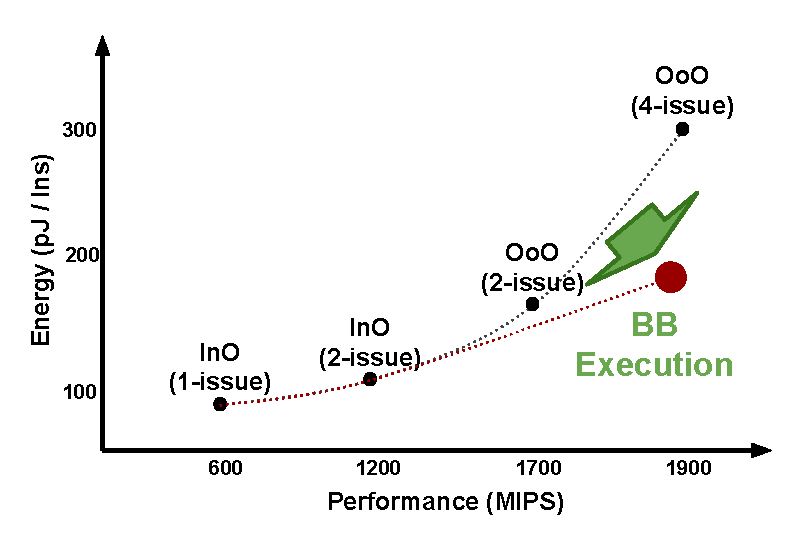
\includegraphics[width=1.0\columnwidth]{fig/energy_perf_insight.pdf} 
    \caption{Energy-Performance trend of recent
        micro-architectures~\cite{azizi2010energy}. The focus of this work is to
            shift this curve towards the lower right corner.}
	\label{fig:insight}
\end{figure}

Section~\ref{sec:rel_work} covers the related work,
    section~\ref{sec:o3_overhead} discusses the major energy bottlenecks of the
    OoO execution, section~\ref{sec:course_grain} describes our energy
    efficiency vision behind coarse-grain execution, section~\ref{sec:code_gen}
    discusses our energy-aware compilation methodology, section~\ref{sec:uarch}
    provides the Bsaic-block execution model microarchitecture,
    section~\ref{sec:simulation} has the simulation methodology,
    section~\ref{sec:discussion} discusses the results achieved in this work,
    and section~\ref{sec:conclusion} concludes the paper.
